\chapter{Mission results}
% During the project, all of the radio system parts have been chosen, measured and verified. The satellite, consisting of the communication module and the folded antennas were integrated. The ground station was built using off-the-shelf radio transceiver with custom designed Low Noise Amplifier.
% The measurement of the sensitivity of the receivers were performed.
% Link budget was calculated to make sure that the link margins are sufficient, using the measured data.

\section{Primary mission}
At $3^{rd}$ of December 2018, PW-Sat2 was launched on \SI{590}{\kilo\meter} orbit on-board Falcon9 rocket from SpaceX company. During the first hours after launch, PW-Sat2 was inside the deployer, completely turned off by the hardware kill-switch. Four hours after the launch, it was deployed, and the system turned on automatically. On-Board software, after the silent period of \SI{40}{\minute} performed antenna deployment procedure and started transmitting beacon data every \SI{60}{\second}. First beacon frame (consisting of satellite telemetry) was received by Scott Chapman (K4KDR) from the United States of America at 6:10 am the day after launch. 

During the first couple of days of orbital operations, the Bus and Payload commissionings were performed by the operators on the ground. At first, the satellite was transmitting with \SI{1200}{\bps} downlink speed, providing reliable radio link. When the basic satellite data was verified, the communication module was switched to \SI{9600}{\bps} to speed up data transfer and reduce power consumption. PW-Sat2 took first polish satellite photograph and transferred to the ground stations at $5^{th}$ of December 2018 (fig. \ref{sat_photo}). It was taken by a part of camera built-in tests and downloaded on request from the ground.

\begin{figure}[H]
    \centering
    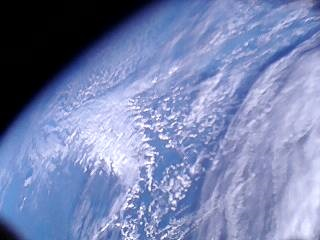
\includegraphics[width=0.5\paperwidth]{img/9/sat_photo.jpg}
    \caption{First polish satellite photo, taken of $5^{th}$ of Decemer 2018}
    \label{sat_photo}
\end{figure}

During the launch, \si{64} satellites were launched together and were separated from the upper stage of the rocket by spring actions. At first, they were flying together, and with time, they were further apart from each other. Figure \ref{25_days} show the on-orbit position of the satellites on \si{25^{th}} day after the launch. Doppler effect estimation was performed during every pass, with increased accuracy. The typical method for selecting a satellite object from a set of different ones is done by applying Doppler correction to the received signal spectrum, for every object in the field of view, and later choosing the most suited one. Signal before and after Doppler correction is shown in the figure \ref{Doppler_correction_gqrx}.

\begin{figure}[H]
    \centering
    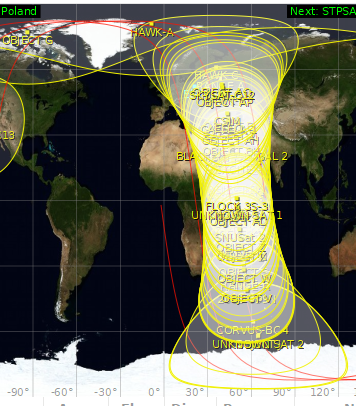
\includegraphics[width=0.4\paperwidth]{img/9/25_days.png}
    \caption{Satellites after \si{25} days after deployment}
    \label{25_days}
\end{figure}

\begin{figure}[H]
    \centering
    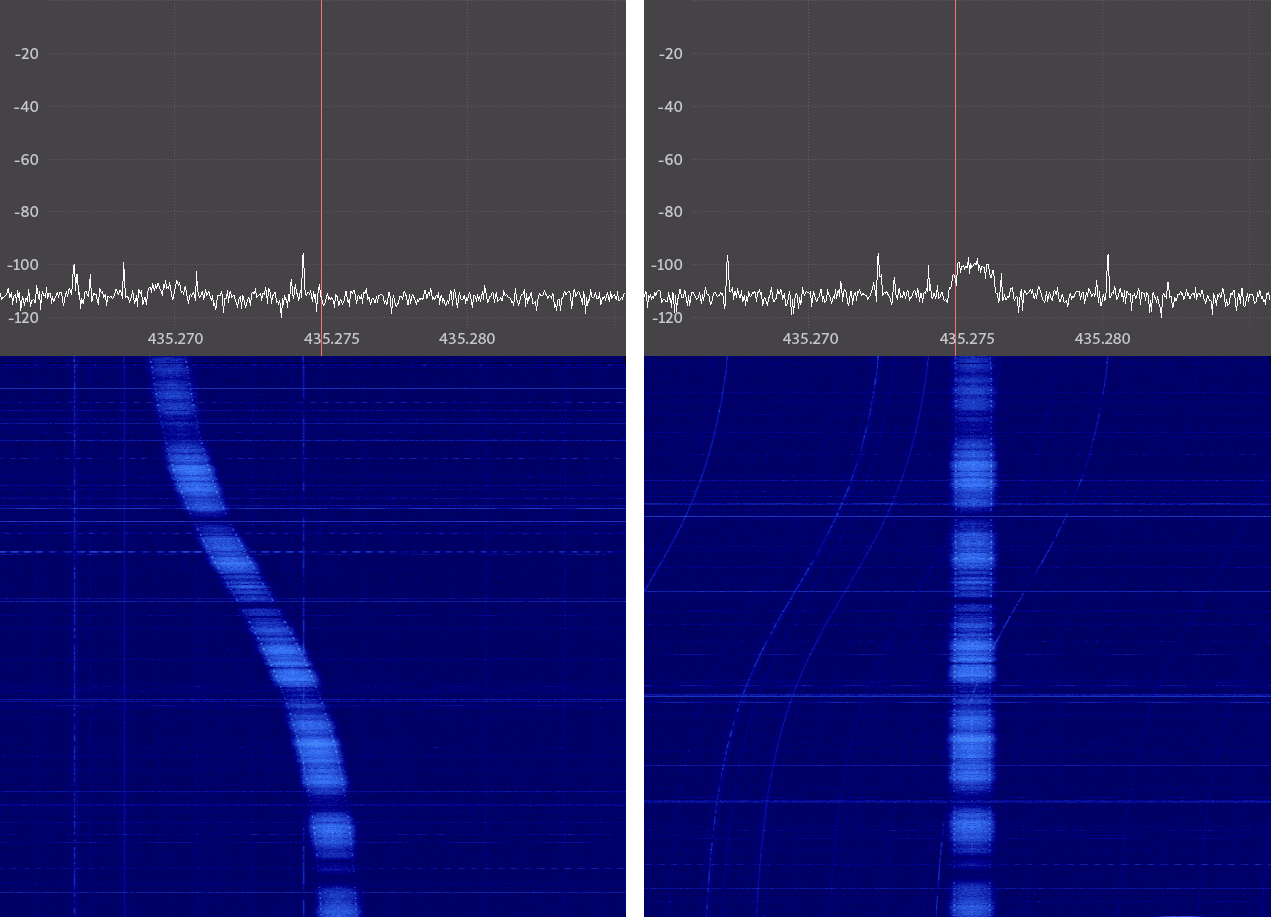
\includegraphics[width=0.5\paperwidth]{img/9/doppler_correction.png}
    \caption{Doppler correction}
    \label{Doppler_correction_gqrx}
\end{figure}

During its primary mission, PW-Sat2 executed \si{157} communication sessions with the ground stations, executing all the experiments more times than planned. It also sent telemetry data to the ground, providing full \SI{24}{\hour} telemetry coverage. For example, the temperature graph from 26th of December 2018 is shown in figure \ref{onboard_temps}. During the end of this phase, PW-Sat2 opened its deorbit sail, capturing video footage and sending it online to the ground.

\begin{figure}[H]
    \centering
    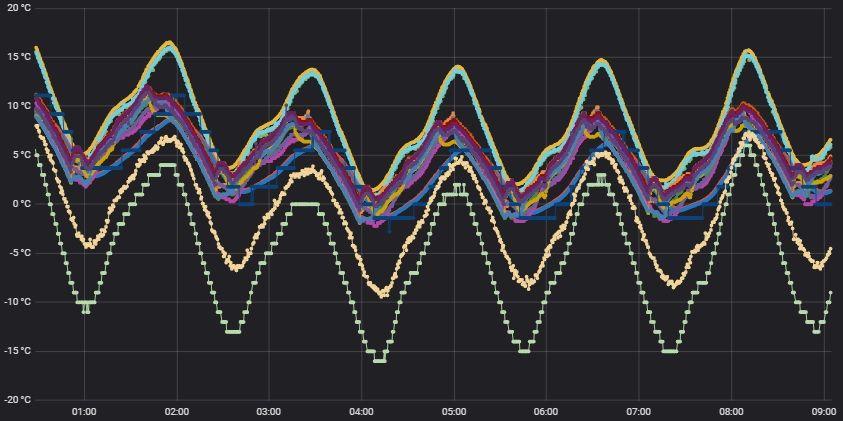
\includegraphics[width=0.65\paperwidth]{img/9/temps_24_12.jpg}
    \caption{On-Board temperatures on $24^{th}$ of December 2018}
    \label{onboard_temps}
\end{figure}

\section{Extended mission}
During the extended mission, PW-Sat2 is continuously monitored via its radio link by the operators. Additional Sun Sensor and RadFET experiment are being executed every two weeks, with additional photographs of the deorbit sail. The state of the sail (fig. \ref{sail_photo}) is monitored to verify its degradation and to compare the deorbitation speed with the simulations (fig. \ref{deorbitation}). During all the satellite passes, automatic tools are checking the system status.

\begin{figure}[H]
    \centering
    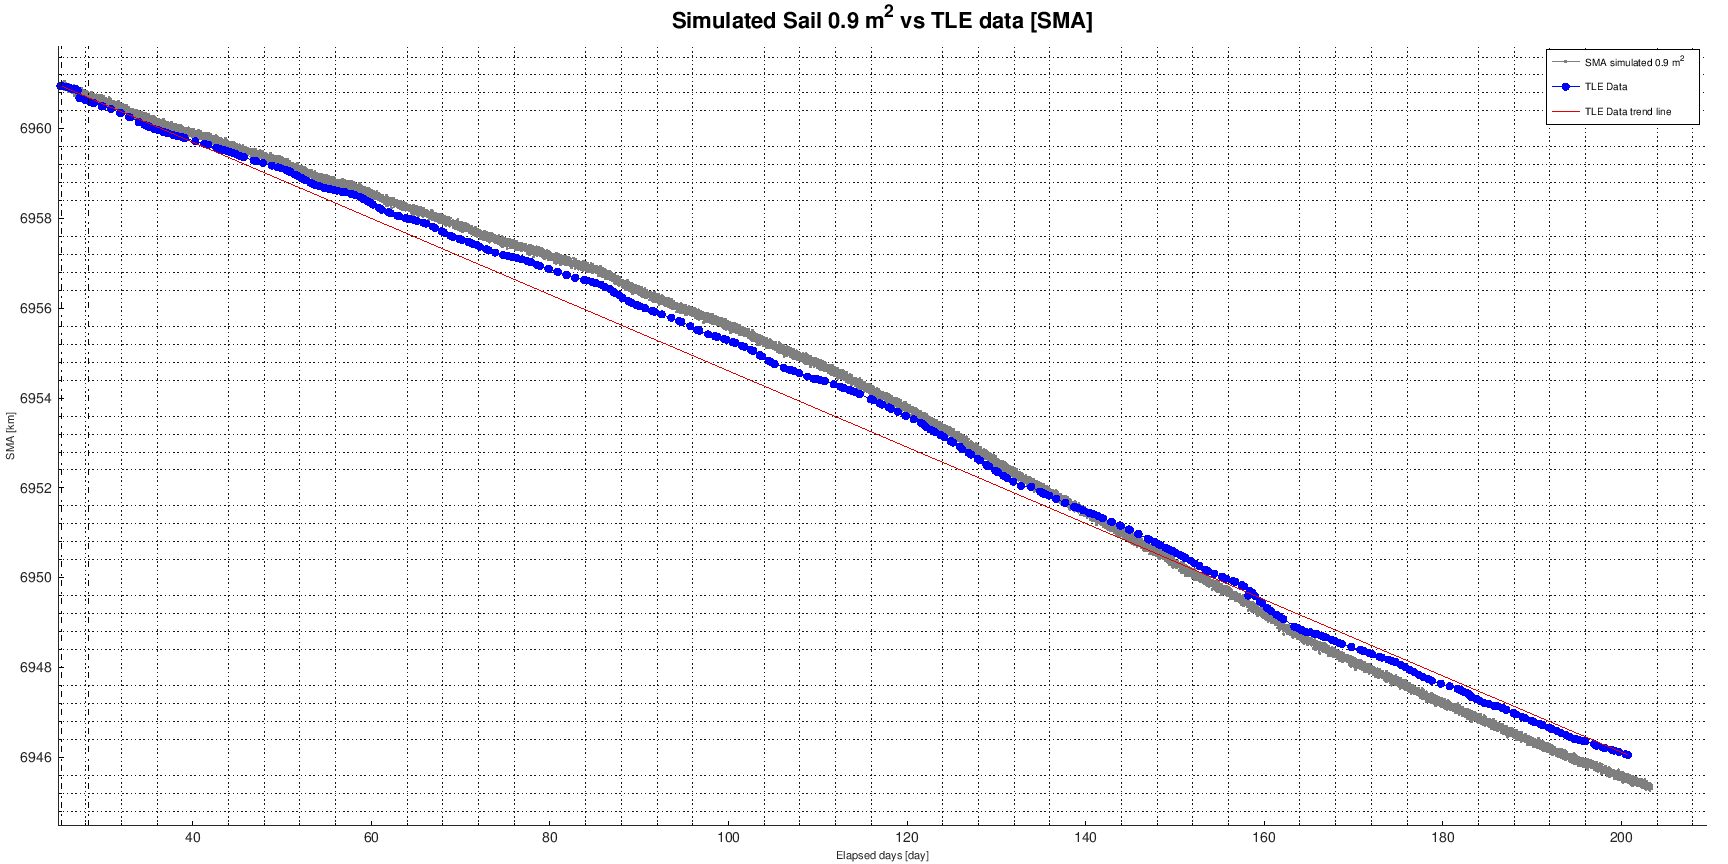
\includegraphics[width=0.65\paperwidth]{img/9/deorbitation.png}
    \caption{PW-Sat2 deorbitation}
    \label{deorbitation}
\end{figure}

\section{Summary}
This thesis described the challenges and requirements for building a CubeSat communication system. All of the design has been verified on the ground by various tests, calculations and predictions. Full end-to-end tests verified the correctness of the bought and designed components. The final test, during the satellite deployment and operations, proving the correctness of the designed radio link.

Since $3^{rd}$ of December, PW-Sat2 is continuously communicating with its ground stations, sending telemetry data and performing experiments. Thanks to the radio link the main mission was a success, delivering video footage from the sail opening. Up to date (25.06.2019), $15^{th}$ RadFET run has been performed, with $7^{th}$ Sun Sensor experiments. Satellite, on the commands from operators, took \si{572} photographs and sent them to Earth. \si{1343} communication sessions were executed, and during which, \SI{95.7}{\percent} of them the two-way communication was successfully established. At total, \SI{26.3}{\mega\byte} of data was sent to the ground.

\begin{figure}[H]
    \centering
    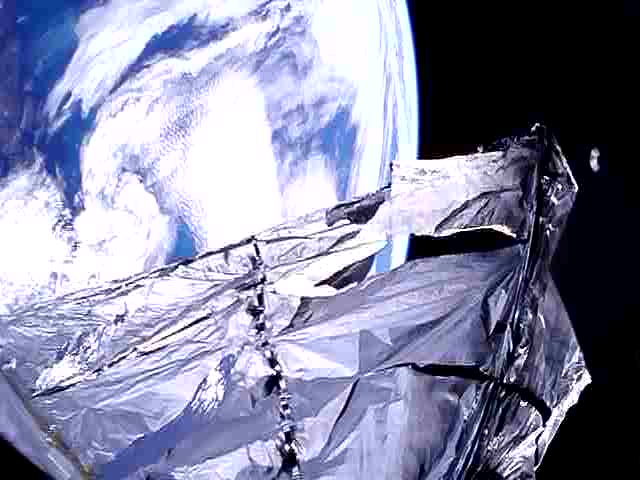
\includegraphics[width=0.65\paperwidth]{img/9/sail_photo.jpg}
    \caption{Sail photograph taken on 16.06.2019}
    \label{sail_photo}
\end{figure}